\section{Problem: Forest fire}
Wildfires in some countries can be a huge problem. Devastating forests, plantations or even habitations, the causes of such fires can be natural or criminal.
Each year wildfires destroy 6 to 14 million hectares of fire-sensitive forests worldwide. Throughout the world, forest fires are out of control. As an example at least one hundred villages are burned every year in Nepal, and some of them are destroyed by forest fires.
In order to prevent these catastrophes, fire lookout towers, public hotlines, ground and aerial patrols are used to detect fire starts. However, this surveillance has to be done day and night in large areas, resulting in high costs and risks for the patrols.

\section{Solution: Drone surveillance}
Early location and identification of fires is needed. A solution to improve the actual surveillance could be the use drones in order to fly long distances and cover large areas to find forest fires in an incipient stage. Also, this will minimize risks and time spent on such operations. 

\subsection{Project Scope}
\begin{itemize}  
        \item Assure permanent connection between drone and GNS
        \item Use directional antennas for both drone and GNS 
        \item Control both antennas to have maximum directivity (pointing directly at each other)
\end{itemize}

\subsection{Constraints}
\begin{itemize}  
        \item Limited frequency and bandwidth by means of the Law
        \item Limited antenna power and size
\end{itemize}

\subsection{Scenario parameters}
We assume that the risk area that the drone will cover is a rectangle:
\begin{equation*}\label{eq:scenario_parameters1} 
 		A_{zone} = xy
\end{equation*}

\begin{figure}[hb]
  	\centering
 	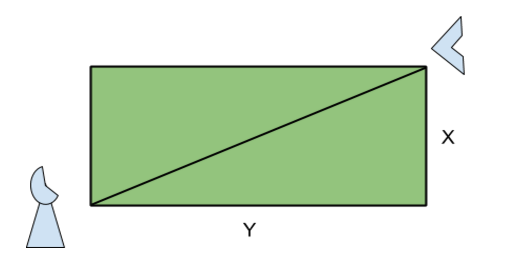
\includegraphics[width=0.8\textwidth]{figures/pic1.png}
  	\caption[Pipeline survey]{Scenario}
\end{figure}

Given the area of the rectangle we can compute the maximum distances of communication, which is the diagonal of the rectangle: 
\begin{equation*}\label{eq:scenario_parameters2} 
 		d_{max} = \sqrt{x^2 + y^2}
\end{equation*}
This distance will be taken into account when computing the radio link communication between the drone and GNS.
